\documentclass[11pt]{article}

%FOR SCRIBES: Please change the next three lines to reflect the correct
%FOR SCRIBES: lecture number, name, and date.
\newcommand{\lecturenumber}{7}
\newcommand{\scribename}{{Linear Transformations and it's Applications}}

\usepackage{subfigure}
\usepackage{hyperref} 
\usepackage{color}
\usepackage{url}
\usepackage{graphicx}
\usepackage{fullpage}
\usepackage{mathtools}
\newcommand{\etal}{{\em et al.}}
\newcommand{\qed}{\mbox{}\hspace*{\fill}\nolinebreak\mbox{$\rule{0.6em}{0.6em}$}}
\newcommand{\expect}{{\bf \mbox{\bf E}}}
\newcommand{\prob}{{\bf \mbox{\bf Pr}}}

%--------------------------- Commands and Environments I added -----------------
\usepackage[english]{babel}
\usepackage{amssymb}
\usepackage{amsmath}
\usepackage{fancyhdr}
\usepackage{tikz}
\renewcommand{\baselinestretch}{1.10}
%%      Fonts:
%%---------------------------------------------------------------------------
\newfont{\bssten}{cmssbx10}
\newfont{\bssnine}{cmssbx10 scaled 900}
\newfont{\bssdoz}{cmssbx10 scaled 1200}

%---------------------------------------------------------------------------
\newcounter{topic} \setcounter{topic}{0}
\newcommand{\topic}[1]{\par \refstepcounter{topic} {\bssdoz \arabic{topic}.~ #1} \par}
%\newcommand{\topic}[1]{\par \refstepcounter{topic} \vs{2ex} {\bssdoz \arabic{topic}.~ #1} \par \vs{1ex}}

%------------------------------ end of new commands and evironments ------------

\definecolor{gray}{rgb}{0.5,0.5,0.5}
\newcommand{\comment}[1]{{\color{gray}[\textsf{#1}]}}
\newcommand{\redospace}{\small\renewcommand{\baselinestretch}{1.5}\normalsize}
\newcommand{\undospace}{\small\renewcommand{\baselinestretch}{1}\normalsize}
\newtheorem{theorem}{Theorem}[section]
\newtheorem{lemma}[theorem]{Lemma}
%----------------------------- some other things I added ---------------------
\newtheorem{claim}[theorem]{Claim}
\newtheorem{example}[theorem]{Example}
\newtheorem{protocol}[theorem]{Protocol}
%----------------------------------------------------------------------------
\newtheorem{corollary}[theorem]{Corollary}
\newtheorem{definition}{Definition}[section]
\newtheorem{remark}[definition]{Remark}
\newtheorem{conjecture}[theorem]{Conjecture}
\newtheorem{proposition}[theorem]{Proposition}
\newenvironment{proof}{{\bf Proof:}}{$\qed$\par}
\newenvironment{proofof}[1]{{\bf Proof of #1:}}{$\qed$\par}
\newenvironment{proofsketch}{{\sc{Proof Outline:}}}{$\qed$\par}

\usepackage{hyperref}
\hypersetup{
	bookmarksnumbered
}


	
	\begin{document}
		%{	\color{blue}   \textbf{Edit the parts in blue and remove this part}}
		\begin{center}
			\framebox{\parbox{6.5in}{
					{\bf{ELL780  Indian Institute of Technology Delhi} }\\ 
					{\bf  {\color{blue} Lecture 7\; {Linear Transformations and it's Applications}}}
					\\
					{Scribed by: {\color{blue}\textit{Chinmay Rjpurohit, Shailesh Mishra}}\\ Instructor:
						 Prof. Sandeep Kumar}
			}}
			\ \\
		\end{center}
%		\noindent{\bf Note}: {LaTeX template courtesy of UC Berkeley EECS dept.}
		
		\noindent {\bf Disclaimer}: {These notes have not been subjected to the
			usual scrutiny reserved for formal publications.  They may be distributed
			outside this class only with the permission of the Course Coordinator.}
		\vspace*{4mm}
		\setcounter{section}{\lecturenumber}
		%FOR SCRIBES: ---------- Begin Scribing Here ------------------------
	\paragraph{"Unfortunately, no one can be told what the Matrix is. You have to see it for yourself." - Morpheus }
    

\section{\textbf{Introduction}}
Linear transformations are fundamental concepts in linear algebra that describe how vectors are mapped from one vector space to another while preserving operations of addition and scalar multiplication. They provide the mathematical framework for numerous applications across physics, computer graphics, data science, and engineering. 

\section{\textbf{Definition and Intuition}}

A \textbf{linear transformation} \( T: \mathbb{R}^n \to \mathbb{R}^m \) is a mapping that satisfies the following properties:

\begin{enumerate}
    \item \textbf{Additivity:} 
    \[
    T(\mathbf{u} + \mathbf{v}) = T(\mathbf{u}) + T(\mathbf{v}) \quad \text{for all } \mathbf{u}, \mathbf{v} \in \mathbb{R}^n.
    \]
    \item \textbf{Homogeneity:} 
    \[
    T(c\mathbf{u}) = cT(\mathbf{u}) \quad \text{for all } c \in \mathbb{R}, \mathbf{u} \in \mathbb{R}^n.
    \]
\end{enumerate}

Linear transformations preserve the linear structure of vector spaces, which makes them essential in both pure and applied mathematics.

\subsection*{Intuition}

Linear transformations can be visualized as actions that stretch, compress, rotate, or shear vector spaces. For example:
\begin{itemize}
    \item A transformation that rotates a square in \( \mathbb{R}^2 \) will map it to another rotated square, preserving linearity.
    \item A projection maps vectors onto a line or plane, reducing the dimension while retaining structure.
\end{itemize}

The following diagram shows how a matrix \( A = \begin{bmatrix} 2 & 0 \\ 0 & 1 \end{bmatrix} \) transforms the standard basis vectors \( \mathbf{e}_1 \) and \( \mathbf{e}_2 \):

\begin{center}
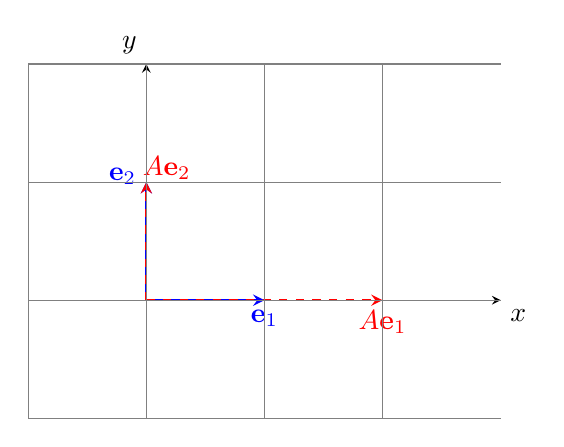
\begin{tikzpicture}[scale=1.5, >=stealth]
    % Axes
    \draw[->] (-1, 0) -- (3, 0) node[anchor=north west] {$x$};
    \draw[->] (0, -1) -- (0, 2) node[anchor=south east] {$y$};
    
    % Original basis vectors
    \draw[->, thick, blue] (0, 0) -- (1, 0) node[anchor=north] {\( \mathbf{e}_1 \)};
    \draw[->, thick, blue] (0, 0) -- (0, 1) node[anchor=east, yshift=2pt] {\( \mathbf{e}_2 \)};
    
    % Transformed basis vectors
    \draw[->, thick, red, dashed] (0, 0) -- (2, 0) node[anchor=north] {\( A\mathbf{e}_1 \)};
    \draw[->, thick, red, dashed] (0, 0) -- (0, 1) node[anchor=west, xshift=-5pt, yshift=5pt] {\( A\mathbf{e}_2 \)};
    
    % Grid lines
    \foreach \x in {-1, 0, 1, 2} {
        \draw[gray, thin] (\x, -1) -- (\x, 2);
    }
    \foreach \y in {-1, 0, 1, 2} {
        \draw[gray, thin] (-1, \y) -- (3, \y);
    }
\end{tikzpicture}
\end{center}

\section{\textbf{Matrix Representation}}

Every linear transformation \( T: \mathbb{R}^n \to \mathbb{R}^m \) can be represented as a matrix \( A \) such that:
\[
T(\mathbf{v}) = A\mathbf{v}, \quad \text{where } A \text{ is an } m \times n \text{ matrix}.
\]

The columns of \( A \) are determined by how \( T \) acts on the basis vectors of \( \mathbb{R}^n \). Specifically:
\[
A = \begin{bmatrix} T(\mathbf{e}_1) & T(\mathbf{e}_2) & \cdots & T(\mathbf{e}_n) \end{bmatrix},
\]
where \( \mathbf{e}_i \) are the standard basis vectors.

\subsection*{Visualization: Effect on Basis Vectors}

The diagram below shows how the transformation matrix \( A = \begin{bmatrix} 2 & 1 \\ 0 & 1 \end{bmatrix} \) maps the basis vectors \( \mathbf{e}_1 = \begin{bmatrix} 1 \\ 0 \end{bmatrix} \) and \( \mathbf{e}_2 = \begin{bmatrix} 0 \\ 1 \end{bmatrix} \):

\begin{center}
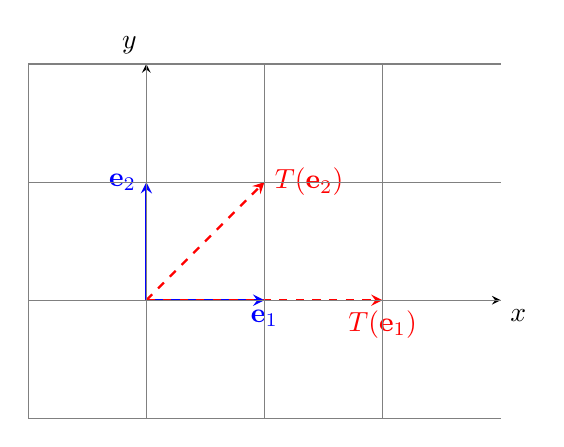
\begin{tikzpicture}[scale=1.5, >=stealth]
    % Axes
    \draw[->] (-1, 0) -- (3, 0) node[anchor=north west] {$x$};
    \draw[->] (0, -1) -- (0, 2) node[anchor=south east] {$y$};
    
    % Original basis vectors
    \draw[->, thick, blue] (0, 0) -- (1, 0) node[anchor=north] {\( \mathbf{e}_1 \)};
    \draw[->, thick, blue] (0, 0) -- (0, 1) node[anchor=east] {\( \mathbf{e}_2 \)};
    
    % Transformed basis vectors
    \draw[->, thick, red, dashed] (0, 0) -- (2, 0) node[anchor=north] {\( T(\mathbf{e}_1) \)};
    \draw[->, thick, red, dashed] (0, 0) -- (1, 1) node[anchor=west] {\( T(\mathbf{e}_2) \)};
    
    % Grid lines
    \foreach \x in {-1, 0, 1, 2} {
        \draw[gray, thin] (\x, -1) -- (\x, 2);
    }
    \foreach \y in {-1, 0, 1, 2} {
        \draw[gray, thin] (-1, \y) -- (3, \y);
    }
\end{tikzpicture}
\end{center}

\subsection*{Key Observations}
1. \( T(\mathbf{e}_1) = \begin{bmatrix} 2 \\ 0 \end{bmatrix} \) becomes the first column of \( A \).
2. \( T(\mathbf{e}_2) = \begin{bmatrix} 1 \\ 1 \end{bmatrix} \) becomes the second column of \( A \).
3. The transformation matrix \( A \) is:
\[
A = \begin{bmatrix} 2 & 1 \\ 0 & 1 \end{bmatrix}.
\]

This shows that the columns of \( A \) encode the action of \( T \) on the basis vectors of the domain.

\section{\textbf{Properties of Linear Transformations}}

Linear transformations possess several key properties that make them fundamental in linear algebra. This section highlights important concepts such as the kernel, range, rank-nullity theorem, and invertibility.

\subsection*{1. Kernel and Range}

- \textbf{Kernel (Null Space)}: The set of all vectors that are mapped to the zero vector under the transformation \( T \):
\[
\text{Ker}(T) = \left\{\mathbf{v} \in \mathbb{R}^n \mid T(\mathbf{v}) = \mathbf{0}\right\}.
\]
The kernel captures directions in the input space that are "flattened" or collapsed to zero by the transformation. It provides insight into the structure of \( T \) and its nullity.

- \textbf{Range (Image)}: The set of all possible outputs of the transformation \( T \):
\[
\text{Im}(T) = \left\{T(\mathbf{v}) \mid \mathbf{v} \in \mathbb{R}^n\right\}.
\]
The range represents the span of the columns of the transformation matrix \( A \). It defines the subspace of \( \mathbb{R}^m \) that the transformation \( T \) maps onto.


\subsubsection*{Visualization: Kernel and Range}

The diagram below shows the kernel and range for a linear transformation \( T: \mathbb{R}^2 \to \mathbb{R}^2 \) represented by \( A = \begin{bmatrix} 1 & 1 \\ 0 & 0 \end{bmatrix} \).

\begin{center}
\begin{tikzpicture}[scale=1.5, >=stealth]
    % Axes
    \draw[->] (-2, 0) -- (2, 0) node[anchor=north] {$x$};
    \draw[->] (0, -1) -- (0, 2) node[anchor=east] {$y$};
    
    % Dashed lines indicating kernel and range directions
    \draw[dashed, gray] (-1.5, 1.5) -- (1.5, -1.5); % Line y = -x (Kernel)
    \draw[dashed, gray] (-2, 0) -- (2, 0); % x-axis (Range)
    
    % Kernel vectors
    \draw[->, thick, blue] (0, 0) -- (-1, 1);
    \draw[->, thick, blue] (0, 0) -- (1, -1);
    % Label for Kernel
    \node[blue, anchor=south east] at (-1, 1) {\( \text{Ker}(T) \)};
    
    % Range vector
    \draw[->, thick, red] (0, 0) -- (1.5, 0);
    % Label for Range
    \node[red, anchor=north east] at (1.5, 0.1) {\( \text{Im}(T) \)};
\end{tikzpicture}
\end{center}


\subsection*{2. Rank-Nullity Theorem}

The \textbf{Rank-Nullity Theorem} provides a fundamental relationship between the dimensions of the kernel and the range:
\[
\text{dim}(\text{Ker}(T)) + \text{dim}(\text{Im}(T)) = n,
\]
where \( n \) is the dimension of the domain of \( T \). This theorem connects the nullity (dimension of the kernel) and the rank (dimension of the range) of a transformation.

\subsection*{3. Invertibility}

A linear transformation \( T \) is invertible if and only if:
\begin{itemize}
    \item \( \text{Ker}(T) = \{\mathbf{0}\} \) (injective).
    \item \( \text{Im}(T) = \mathbb{R}^m \) (surjective).
    \item The determinant of the transformation matrix \( \det(A) \neq 0 \).
\end{itemize}

For an invertible transformation:
\[
T^{-1}(T(\mathbf{v})) = \mathbf{v}, \quad \forall \mathbf{v} \in \mathbb{R}^n.
\]

\subsection*{4. Composition of Transformations}

If \( T_1: \mathbb{R}^n \to \mathbb{R}^m \) and \( T_2: \mathbb{R}^m \to \mathbb{R}^p \) are linear transformations, their composition \( T_2 \circ T_1 \) is also a linear transformation. The associated matrix satisfies:
\[
A_{T_2 \circ T_1} = A_{T_2} A_{T_1}.
\]
This property is widely used in applications like computer graphics and machine learning.

\subsection*{5. Determinant and Orientation}

The determinant of the transformation matrix \( A \):
\begin{itemize}
    \item Indicates the scaling factor of areas (in \( \mathbb{R}^2 \)) or volumes (in \( \mathbb{R}^3 \)) under \( T \).
    \item Determines whether \( T \) preserves orientation (\( \det(A) > 0 \)) or reverses it (\( \det(A) < 0 \)).
    \item If \( \det(A) = 0 \), the transformation collapses the space into a lower dimension, and \( T \) is not invertible.
\end{itemize}

\subsection*{6. Linear Independence Preservation}

A linear transformation preserves the linear independence of vectors if \( T \) is injective (one-to-one), which occurs when \( \text{Ker}(T) = \{\mathbf{0}\} \).

\section*{Summary}

Linear transformations elegantly unify the algebraic and geometric understanding of vector spaces. Their properties, such as kernel, range, rank, and invertibility, provide critical insights into their behavior and applications.

\section{\textbf{Geometric Transformations}}

Linear transformations in \( \mathbb{R}^2 \) can be understood geometrically as operations that alter the shape or orientation of objects while preserving linearity. Here are five common geometric transformations:

\subsection*{1. Scaling}
Scaling uniformly enlarges or shrinks vectors. It is represented by a diagonal matrix:
\[
A = \begin{bmatrix} k & 0 \\ 0 & k \end{bmatrix}, \quad k > 0.
\]
If \( k > 1 \), the object is stretched; if \( 0 < k < 1 \), the object is compressed.

\begin{center}
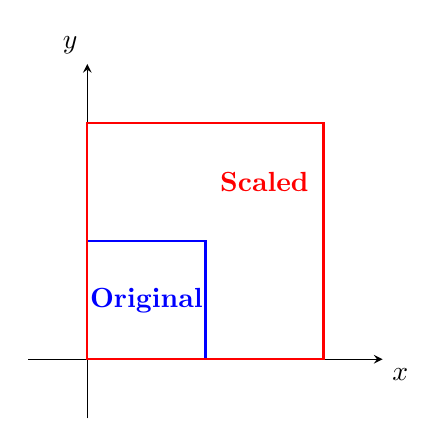
\begin{tikzpicture}[scale=1.5, >=stealth]
    % Axes
    \draw[->] (-0.5, 0) -- (2.5, 0) node[anchor=north west] {$x$};
    \draw[->] (0, -0.5) -- (0, 2.5) node[anchor=south east] {$y$};
    
    % Original square
    \draw[thick, blue] (0, 0) -- (1, 0) -- (1, 1) -- (0, 1) -- cycle;
    \node[blue] at (0.5, 0.5) {\textbf{Original}};
    
    % Transformed square
    \draw[thick, red] (0, 0) -- (2, 0) -- (2, 2) -- (0, 2) -- cycle;
    \node[red] at (1.5, 1.5) {\textbf{Scaled}};
\end{tikzpicture}
\end{center}

---

\subsection*{2. Rotation}
Rotation rotates vectors counterclockwise by an angle \( \theta \). The rotation matrix is:
\[
R = \begin{bmatrix} \cos\theta & -\sin\theta \\ \sin\theta & \cos\theta \end{bmatrix}.
\]

For example, a rotation by \( 45^\circ \) (\( \theta = \pi/4 \)) is shown below:

\begin{center}
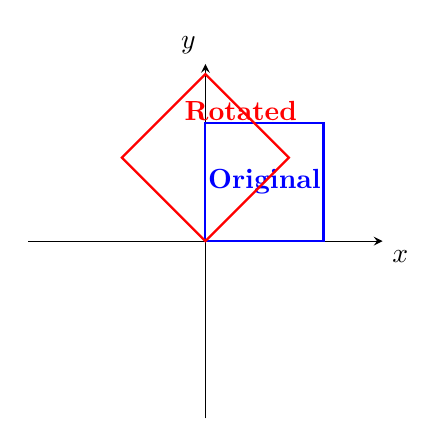
\begin{tikzpicture}[scale=1.5, >=stealth]
    % Axes
    \draw[->] (-1.5, 0) -- (1.5, 0) node[anchor=north west] {$x$};
    \draw[->] (0, -1.5) -- (0, 1.5) node[anchor=south east] {$y$};
    
    % Original square
    \draw[thick, blue] (0, 0) -- (1, 0) -- (1, 1) -- (0, 1) -- cycle;
    \node[blue] at (0.5, 0.5) {\textbf{Original}};
    
    % Rotated square
    \draw[thick, red] (0, 0) -- (0.707, 0.707) -- (0, 1.414) -- (-0.707, 0.707) -- cycle;
    \node[red] at (0.3, 1.1) {\textbf{Rotated}};
\end{tikzpicture}
\end{center}

---

\subsection*{3. Reflection}
Reflection flips vectors over a line, such as the \( x \)-axis, \( y \)-axis, or other axes. A reflection over the \( y \)-axis is represented by:
\[
A = \begin{bmatrix} -1 & 0 \\ 0 & 1 \end{bmatrix}.
\]

\begin{center}
\begin{tikzpicture}[scale=1.5, >=stealth]
    % Axes
    \draw[->] (-2, 0) -- (2, 0) node[anchor=north west] {$x$};
    \draw[->] (0, -0.5) -- (0, 2.5) node[anchor=south east] {$y$};
    
    % Original square
    \draw[thick, blue] (0, 0) -- (1, 0) -- (1, 1) -- (0, 1) -- cycle;
    \node[blue] at (0.5, 0.5) {\textbf{Original}};
    
    % Reflected square
    \draw[thick, red] (0, 0) -- (-1, 0) -- (-1, 1) -- (0, 1) -- cycle;
    \node[red] at (-0.5, 0.5) {\textbf{Reflected}};
\end{tikzpicture}
\end{center}

---

\subsection*{4. Shear}
Shear skews vectors, transforming squares into parallelograms. A shear along the \( x \)-axis is represented by:
\[
A = \begin{bmatrix} 1 & k \\ 0 & 1 \end{bmatrix}.
\]

\begin{center}
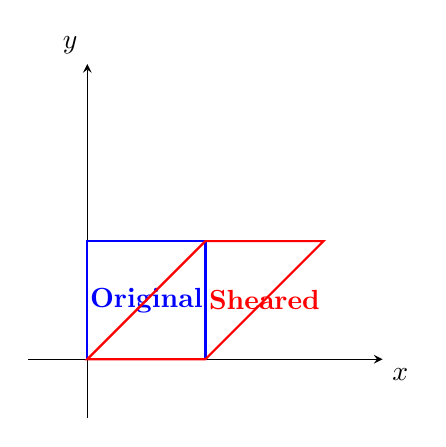
\begin{tikzpicture}[scale=1.5, >=stealth]
    % Axes
    \draw[->] (-0.5, 0) -- (2.5, 0) node[anchor=north west] {$x$};
    \draw[->] (0, -0.5) -- (0, 2.5) node[anchor=south east] {$y$};
    
    % Original square
    \draw[thick, blue] (0, 0) -- (1, 0) -- (1, 1) -- (0, 1) -- cycle;
    \node[blue] at (0.5, 0.5) {\textbf{Original}};
    
    % Sheared square
    \draw[thick, red] (0, 0) -- (1, 0) -- (2, 1) -- (1, 1) -- cycle;
    \node[red] at (1.5, 0.5) {\textbf{Sheared}};
\end{tikzpicture}
\end{center}

---

\subsection*{5. Projection}
Projection maps vectors onto a subspace. For example, projection onto the \( x \)-axis is represented by:
\[
P = \begin{bmatrix} 1 & 0 \\ 0 & 0 \end{bmatrix}.
\]

\begin{center}
\begin{tikzpicture}[scale=1.5, >=stealth]
    % Axes
    \draw[->] (-1, 0) -- (2.5, 0) node[anchor=north west] {$x$};
    \draw[->] (0, -0.5) -- (0, 2) node[anchor=south east] {$y$};
    
    % Original vector
    \draw[->, thick, blue] (0, 0) -- (1, 1) node[anchor=north west] {\( \mathbf{v} \)};
    
    % Projected vector
    \draw[->, thick, red] (0, 0) -- (1, 0) node[anchor=north] {\( P\mathbf{v} \)};
    \draw[dashed] (1, 1) -- (1, 0);
\end{tikzpicture}
\end{center}

\section{\textbf{Eigenvalues and Eigenvectors}} 

Eigenvalues and eigenvectors are critical for analyzing the behavior of linear transformations. They help identify invariant directions and scaling factors.

\subsection*{1. Definitions}

- \textbf{Eigenvector}: A nonzero vector \( \mathbf{v} \) that satisfies the equation:
\[
T(\mathbf{v}) = \lambda \mathbf{v},
\]
where \( \lambda \) is a scalar known as the eigenvalue.

- \textbf{Eigenvalue}: The scalar \( \lambda \) associated with an eigenvector \( \mathbf{v} \). It indicates the scaling factor applied to \( \mathbf{v} \) during the transformation. Eigenvalues can be positive, negative, or zero, depending on the nature of the transformation.


1. Eigenvectors indicate directions that remain unchanged (except for scaling).
2. The eigenvalue \( \lambda \):
   - \( \lambda > 1 \): Stretches the eigenvector.
   - \( 0 < \lambda < 1 \): Compresses the eigenvector.
   - \( \lambda = -1 \): Reverses the eigenvector's direction.
   - \( \lambda = 0 \): Maps the eigenvector to \( \mathbf{0} \), indicating a singular transformation.

---

\subsection*{2. Eigenvector-Eigenvalue Equation}
The eigenvalue problem is expressed as:
\[
A\mathbf{v} = \lambda \mathbf{v}.
\]
Rewriting, we get:
\[
(A - \lambda I)\mathbf{v} = \mathbf{0}.
\]
For nontrivial solutions (\( \mathbf{v} \neq \mathbf{0} \)), the determinant of \( (A - \lambda I) \) must be zero:
\[
\det(A - \lambda I) = 0.
\]
This determinant condition produces the \textbf{characteristic polynomial}, whose roots are the eigenvalues \( \lambda \).

---

\subsection*{3. Visualization}

The diagram below illustrates how a linear transformation affects eigenvectors and other vectors. Each element is explained in detail:

\begin{enumerate}
    \item \textbf{Eigenvector 1 (\( \mathbf{v}_1 \))}:
    \begin{itemize}
        \item Shown in blue.
        \item Transformed into a scaled version (red) by the eigenvalue \( \lambda_1 \) under the linear transformation \( T \).
    \end{itemize}
    
    \item \textbf{Eigenvector 2 (\( \mathbf{v}_2 \))}:
    \begin{itemize}
        \item Another eigenvector, also shown in blue.
        \item Transformed into a scaled version (red) by the eigenvalue \( \lambda_2 \) under \( T \).
    \end{itemize}
    
    \item \textbf{Generic Vector (\( \mathbf{w} \))}:
    \begin{itemize}
        \item A vector not aligned with any eigenvector.
        \item Its transformation (gray dashed) does not align with simple scaling, as it does not share the invariant properties of eigenvectors.
    \end{itemize}
\end{enumerate}

\begin{center}
\begin{tikzpicture}[scale=1.5, >=stealth]
    % Axes
    \draw[->] (-2, 0) -- (2, 0) node[anchor=north west] {$x$};
    \draw[->] (0, -1) -- (0, 2) node[anchor=south east] {$y$};
    
    % Eigenvector 1 and its transformation
    \draw[->, thick, blue] (0, 0) -- (1, 1) node[anchor=south west] {\( \mathbf{v}_1 \)};
    \draw[->, thick, red] (0, 0) -- (1.5, 1.5) node[anchor=east] {\( T(\mathbf{v}_1) \)};
    
    % Eigenvector 2 and its transformation
    \draw[->, thick, blue] (0, 0) -- (1, -1) node[anchor=north west] {\( \mathbf{v}_2 \)};
    \draw[->, thick, red] (0, 0) -- (0.5, -0.5) node[anchor=north east] {\( T(\mathbf{v}_2) \)};
    
    % Generic vector and its transformation
    \draw[->, thick, gray] (0, 0) -- (1, 0.5) node[anchor=south] {\( \mathbf{w} \)};
    \draw[->, thick, gray, dashed] (0, 0) -- (0.8, 1.2) node[anchor=north east] {\( T(\mathbf{w}) \)};
\end{tikzpicture}
\end{center}



---

\subsection*{4. Applications of Eigenvalues and Eigenvectors}

\begin{enumerate}
    \item \textbf{Stability Analysis:}
    \begin{itemize}
        \item Eigenvalues determine stability in dynamical systems.
        \item Negative eigenvalues indicate stable equilibria, while positive ones suggest instability.
    \end{itemize}
    
    \item \textbf{Principal Component Analysis (PCA):}
    \begin{itemize}
        \item Eigenvectors of the covariance matrix represent the principal directions of data variation.
        \item Eigenvalues indicate the variance captured by each principal component.
    \end{itemize}
    
    \item \textbf{Mechanical Vibrations:}
    \begin{itemize}
        \item Eigenvalues correspond to natural frequencies of vibrating systems.
        \item Eigenvectors describe the modes of vibration.
    \end{itemize}
    
    \item \textbf{Markov Chains:}
    \begin{itemize}
        \item The steady-state distribution corresponds to the eigenvector with eigenvalue 1.
        \item Eigenvalues describe the rates at which the system converges to the steady state.
    \end{itemize}
\end{enumerate}


---

\subsection*{5. Summary}

Eigenvalues and eigenvectors are fundamental tools for analyzing the behavior of linear transformations. They identify invariant directions (eigenvectors) and corresponding scaling factors (eigenvalues), offering insights into the geometry and algebra of transformations. These concepts are crucial in solving problems across various fields, including mathematics, physics, engineering, data science, and computer graphics.



\section{\textbf{Applications of Linear Transformations}} 

Linear transformations are versatile tools that find applications in a wide range of disciplines, including mathematics, computer science, physics, and engineering. Below are some key areas where linear transformations play a pivotal role:


\subsection*{1. Data Science and Machine Learning}

Linear transformations are fundamental to many data analysis and machine learning techniques. They enable the preprocessing and representation of data in meaningful ways. Examples include:

\begin{itemize}
    \item \textbf{Principal Component Analysis (PCA)}:
    A technique to reduce data dimensionality by identifying principal directions of variation (eigenvectors). PCA projects data onto a lower-dimensional subspace while preserving the most significant variance.

    \item \textbf{Feature Transformation}:
    Preprocessing methods like standardization, normalization, and whitening use linear transformations to scale or decorrelate features, making data more suitable for machine learning algorithms.
\end{itemize}


\subsection*{2. Physics and Engineering}

Linear transformations are widely used in physics and engineering to model, analyze, and solve complex systems. They provide a mathematical framework to describe the relationships between physical quantities. Applications include:

\begin{itemize}
    \item \textbf{Stress and Strain Analysis}:
    Tensors representing stress and strain are modeled as linear transformations that relate forces applied to a material to the resulting deformations. These transformations are critical in understanding material properties and structural mechanics.

    \item \textbf{Quantum Mechanics}:
    Operators in Hilbert spaces, such as the Hamiltonian, represent linear transformations that describe the evolution and measurable properties of quantum states. These transformations are central to solving the Schrödinger equation.

    \item \textbf{Electrical Circuits}:
    Transformation matrices are used to model the relationships between voltages, currents, and impedances in circuit networks. This facilitates the analysis and simulation of complex electrical systems.
\end{itemize}


\subsection*{3. Signal Processing}

Linear transformations play a vital role in signal processing, enabling the analysis, decomposition, and manipulation of signals. Applications include:

\begin{itemize}
    \item \textbf{Fourier Transform}:
    A linear transformation that decomposes signals into their frequency components. It is widely used in audio processing, image compression, and communication systems.

    \item \textbf{Image Filters}:
    Convolutional filters, such as edge detection and blurring, are implemented as linear operations applied to pixel intensities. These transformations are essential in image enhancement and computer vision.
\end{itemize}


\subsection*{4. Graph Theory and Networks}

Linear transformations are fundamental in graph theory and network analysis, where matrices represent relationships and structures in graphs. Common examples include:

\begin{itemize}
    \item \textbf{Network Analysis}:
    Eigenvalues of graph Laplacians provide critical insights into graph properties such as connectivity, clustering, and community detection. For example, the second smallest eigenvalue (the Fiedler value) is used to measure graph connectivity.

    \item \textbf{PageRank Algorithm}:
    Google's PageRank algorithm leverages the eigenvectors of the adjacency matrix (or transition matrix) of a web graph to rank web pages by importance. The steady-state eigenvector corresponds to the page ranks.
\end{itemize}


\subsection*{Summary}
Linear transformations are indispensable in both theoretical and practical settings. Their ability to map, rotate, scale, and project vectors underpins countless applications across science, technology, and industry.


\section{\textbf{Conclusion}}  

Linear transformations are fundamental to the study of mathematics, physics, engineering, and numerous other fields. They provide a powerful framework for understanding the relationship between abstract vector spaces and concrete real-world applications. By preserving linearity, they offer insights into the geometric and algebraic structures underlying various systems.

From analyzing eigenvalues and eigenvectors to solving complex systems in physics and engineering, linear transformations serve as a bridge between theory and practice. Their versatility enables advancements in data science, computer graphics, signal processing, and more.

In essence, linear transformations unify diverse concepts and applications under a common mathematical language, making them an indispensable tool in both academic and applied disciplines.



\section*{References}

\begin{enumerate}
    \item Axler, Sheldon. \textit{Linear Algebra Done Right}. Springer, 2015.
    \item Strang, Gilbert. \textit{Introduction to Linear Algebra}. Wellesley-Cambridge Press, 2016.
    \item 3Blue1Brown. \textit{Essence of Linear Algebra} Available at: 
    \href{https://www.3blue1brown.com/essence-of-linear-algebra}{https://www.3blue1brown.com/essence-of-linear-algebra}.
\end{enumerate}

	
\end{document}